\documentclass[12pt, a4paper]{article}%
\usepackage[utf8]{inputenc}
\usepackage[english]{babel}
\usepackage{graphicx}
\usepackage{amssymb}
\usepackage{amsmath}
\usepackage{geometry}
\usepackage{float} 
%\usepackage{tabularray}
\usepackage{array}
%\usepackage{multirow}
\usepackage[table]{xcolor}
\usepackage{tikz}
\usetikzlibrary{positioning, arrows.meta, calc}
%\usepackage{booktabs} 
\renewcommand{\thesubsection}{\thesection.\alph{subsection}}


% bibliography
\usepackage[
    backend=biber,
    style=bwl-FU,
    url=false,
    doi=false,
    eprint=false
]{biblatex}
\addbibresource{literature.bib}

\usepackage{hyperref} %Must be loaded at the end.


\begin{document}

%---------------------------------------------------
%
%%%%%%%%%%%%%%%%%%% front page %%%%%%%%%%%%%%%%%%%%%%%
%
%---------------------------------------------------

\begin{titlepage}

\setlength{\topmargin}{0.5cm}
% \setlength{\bottommargin}{0.1cm}

\center

{\Large \bfseries Do ESG factors relate to yields of companies?
}\\[0.5cm] 

Mariia Kuzmina \footnote{\texttt{mariia.kuzmina@uzh.ch}},
Timon Gehrig \footnote{\texttt{timon.gehrig@bf.uzh.ch}},
Jennifer Li \footnote{\texttt{jennifer.li@execed.uzh.ch}},
Miroslav Zivanovic \footnote{\texttt{miroslav.zivanovic@uzh.ch}}\\
\today
\\ [2cm]

\begin{abstract}
    In this project, we employ the Fama and French 3-Factor Model to analyze the relationship between market risk, size, value on monthly returns for Nasdaq 100 constituents. Further, we examine the effects of incorporating an ESG factor into the factor model.
    The results indicate negative betas for market risk and size, suggesting that high returns cannot be solely achieved through systematic risk. Additionally, the inclusion of the ESG factor shows a positive coefficient, suggesting that companies with superior ESG standards may outperform, although statistical significance remains limited.
    Further research with an extended time period and larger sample size may enhance the robustness of these findings.
\end{abstract}

\vspace{3cm}



\vfill 
\end{titlepage}

\tableofcontents


%---------------------------------------------------
%
%%%%%%%%%%%%%%%%%%% Intro %%%%%%%%%%%%%%%%%
%
%---------------------------------------------------
\newpage
\section{Introduction}
In this research project, we assess the factors introduced by \textcite{FamaFrench1992}. Additionally, we incorporate Environmental, Social, and Governance [ESG] factors into the factor models.
The question arises whether these are valuable factors. Based on this, we examine following research question: How do ESG factors relate to yields of companies?

%---------------------------------------------------
%
%%%%%%%%%%%%%%%%%%%%%% Main sections %%%%%%%%%%%%%%%%%%%%%%%
%												   
%---------------------------------------------------
\section{Factor Models and ESG in existing research}
There exist various approaches to modeling asset prices. One central theory backed by the assumption of investor's rationality is the Efficient Market Hypothesis. It states that all information about a firm value is reflected by its stock price. Accordingly, generating excess returns in terms of alpha is not possible (\textcite{Fama1970}). 

Based upon this, \textcite{Sharpe1964} and \textcite{Lintner1965} introduced the Capital Asset Pricing Model [CAPM]. Given the systematic risk of a stock or a portfolio, the expected return can be calculated. Respectively, the only factor is the beta which represents the market risk. This inevitably leads to anomalies caused by the model, suggesting the need for more factors.

As an alternative, the Arbitrage Pricing Theory [APT] was developed by \textcite{Ross1976} which loosens the assumption that markets are perpetually efficient. Instead, security prices may deviate from the fair value occasionally. However, these temporary mispricings are eventually corrected by market action, making arbitrage opportunities only possible in the short term.
The multi-factor asset pricing models use the idea that there is a linear relationship between the macroeconomic factors and the expected return.

\textcite{FamaFrench1992} have proposed some factors based on the anomalies that were noticed in the CAPM.
First of all, Small-Cap stocks seemingly yield higher expected returns compared to the market which justifies the extension of a size factor called Small Minus Big [SMB].

Additionally, the value anomaly was observed where stocks with a high book-to-market ratio tend to perform better than the market, introducing the High Minus Low [HML] factor.
This leads to the Fama and French Three Factor Model with the two additional factors SMB and HML.

In recent years, ESG factors have gained significant attention in the financial landscape and has emerged as a key determinant of a company’s financial performance. Fama and French's Three-Factor model, which considers risk factors including market risk, size, and value to predict returns, has been integral to yield analysis. To this model, we integrate ESG elements.
Correlating ESG factors with yields is sensible, given that companies with superior ESG standards may achieve higher operational efficiency, establish better stakeholder relationships, and move towards overall risk reduction. These factors could contribute to a stronger financial profile, and by extension, higher yields. Conversely, companies displaying inadequate ESG measures could face operational risks and regulatory sanctions, leading to lower yields.

\section{Methodology}
The data that is observed ranges from September 1st, 2014 to September 1st, 2022 and consists of the constituents of the Nasdaq 100. The constitutents are fetched using Wikipedia as the source.
The \textcite{FamaFrench1992} factors are obtained from the official website, by fetching a complete CSV of monthly factor returns.
Monthly returns and ESG scores of the constituents of the specific index were fetched via Yahoo Finance.\\

These data sets were cleaned by dropping columns consisting of only NA values and implementing the fill-forward method to fill missing values.

\section{Model}
Using the approach based on the \textcite{FamaFrench1992} procedure, the 3-factor model is used. We thus obtain following regression equation:\\
\begin{equation} 
E(r_i) = r_i + \beta(r_M-r_f) + \beta_{SMB} \cdot\text{SMB} +  \beta_{HLM} \cdot\text{HML}
 \end{equation}

Additionally, a multiple linear regressions is performed where monthly returns are regressed on the factors of the 3-factor model, together with a factor which respresents the ESG aspects. It combines the E-, S-, and G-Scores. Accordingly, we refer to it as the ESG factor.\\
\begin{equation}
E(r_i) = r_i + \beta(r_M-r_f) + \beta_{SMB} \cdot\text{SMB} +  \beta_{HLM} \cdot\text{HML} +  \beta_{ESG}\cdot\text{ESG}
\end{equation}

Based on those two equations, we obtain following summary statistis for the 3-factor model:
\begin{table}[]
    \begin{tabular}{l|llll}
                & Intercept                      & Market Risk Premium             & SMB                             & HML                             \\
    Coefficient & 1.160*10$^{-2}$ & -4.884*10$^{-4}$ & -5.312*10$^{-3}$ & -2.965*10$^{-3}$ \\
    t-Value     & 1.741                          & -0.946                          & 0.404                           & -0.635                         
    \end{tabular}
    \end{table}

For the 3-factor model and the ESG factor, we get: \\
\begin{table}[]
    \begin{tabular}{llllll}
                & Intercept                       & Market Risk Premium             & SMB                             & HML                             & ESG                            \\
    Coefficient & -5.900*10$^{-2}$ & -8.300*10$^{-5}$ & -6.167*10$^{-3}$ & -3.050*10$^{-3}$ & 1.009*10$^{-3}$ \\
    t-Value     & 0.068                           & -0.968                          & 0.432                           & -0.642                          & 0.010                         
    \end{tabular}
    \end{table}


Further, we plot the returns according to different ESG factor values.\\ % Check if that's correct

% Check if it's compiled correctly
\begin{figure}
    \centering
    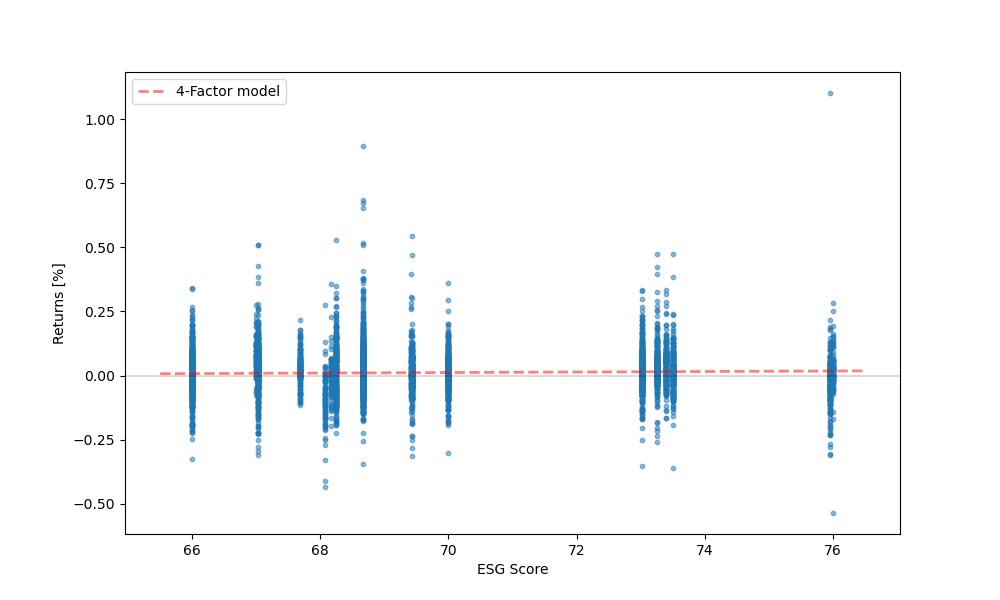
\includegraphics[width=\textwidth]{../figures/regression.png}
    \caption{Regression plot}
    \label{fig:regression}
  \end{figure}

\section{Results} 
When regressing the monthly returns on the \textcite{FamaFrench1992} factors, all the betas for the factors are negative. The market risk premium has a negative regression slope, indicating that there does not exist a premium rewarding systematic risk. The risk-return profile can not be used to get high returns.
The coefficients for SML and HML are both negative, which would mean that the optimal investment strategy is buying stocks issued by large firms, as well as growth stocks.\\
However, as none of the t-values are statistically significant under the 5\% significance level, these results must be handled with caution.\\

Taking the ESG factor is included in the factor model, the dynamics are similar. The only factor exhibiting a positive coefficient is the ESG factor. Hence, high ESG ratings can lead to outperformance.\\
Again, none of the t-values are statistically significant under the 5\% significance level. Thus, there is not a strong enough evidence that our ESG factor relates to yields of companies.
To increase statistical significance, one could increase the inspected time-period. Further, by increasing the sample size, the statistical significance might increase as well. By implementing these robustment enhancements, a stronger relationship may be discovered.


\section{References}
\printbibliography[heading=none]


\end{document}
